\documentclass[11pt]{article}

\usepackage[a4paper,margin=1in]{geometry}
\usepackage{amsmath}
\usepackage{amssymb}
\usepackage{enumitem}
\usepackage{graphicx}
\usepackage{float}

\begin{document}

\begin{center}

{\Large\bfseries
A Workload-Aware Dynamic Array Growth Algorithm for Efficient Memory Allocation
}

\end{center}

\section*{Background}

Dynamic arrays are fundamental data structures widely used in modern software
for fast \mbox{random} access and dynamic memory allocation. Conventional
implementations resize arrays using fixed growth factors (e.g., $1.5\times$
or $2\times$), compromising between memory utilization and \mbox{resizing} \mbox{overhead}
\cite{brodnik}. Though recent studies explore alternative array organizations
to \mbox{improve} \mbox{memory} \mbox{efficiency} \cite{sartor,bille}, the utilized resizing
strategies remain workload-independent, with \mbox{limited} \mbox{flexibility} in adaptation
to changes in insertion patterns. This study proposes an \mbox{adaptive} growth
strategy combining resize history with runtime workload intensity.

\section*{Method}

The proposed algorithm models the growth factor using a workload-aware
harmonic function,

\[
g(k,v)=
\min\left(
g_{\max},
\max\left(
g_{\min},
1+\frac{c_0+\lambda\ln(1+v)}{k}
\right)
\right),
\]

\noindent where $k$ is the resize count and $v = \frac{\Delta N}{\Delta t}$ is
insertion velocity ($\Delta N$ inserted elements per unit time $\Delta t$
between resizes). The resized capacity is $C_{\mathrm{new}} = \lfloor
C_{\mathrm{old}} \times g(k,v) \rfloor$. Implemented in Python 3.11 (64-bit
integers, initial capacity $C_0=10$, $c_0=2.0$, $\lambda=1.0$, $g_{\min}=1.1$,
$g_{\max}=2.0$), benchmarks were run on an Intel i5 Windows 10 workstation
across 10 repeated trials. Evaluation spanned $10^4$--$10^7$ insertions across
seven workload patterns (including uniform, burst, and mixed), comparing
against fixed ($1.5\times, 2.0\times$) and Python list ($1.125\times$)
policies.

\section*{Results and Conclusions}

This study aimed to identify an optimal configuration that minimized memory waste while maintaining high throughput and limiting element-copying overhead. Figure \ref{fig:memory_waste} shows the memory waste comparison across the evaluated resizing strategies. Under a $10^7$
element mixed workload (10 trials), the proposed strategy achieved 1.28\% memory waste, 32 resizes,
38.76M copied elements, and 6.40M ops/s throughput. Comparatively, Fixed
2.0$\times$ yielded 4.63\% waste (20 resizes, 10.49M copies), Fixed 1.5$\times$
yielded 27.77\% waste (35 resizes, 27.69M copies), and Python list yielded
4.59\% waste (102 resizes, 83.84M copies). The proposed method significantly
reduced memory waste compared to fixed and feedback-unaware baselines
($p < 0.01$) without sacrificing throughput. By combining resize history and
workload awareness, the algorithm expands aggressively during burst insertions
and adopts conservative growth during lighter workloads. Unlike static resizing
policies, this work contributes a workload-sensitive adaptive resizing
mechanism for memory-sensitive systems.

\begin{figure}[H]
\centering
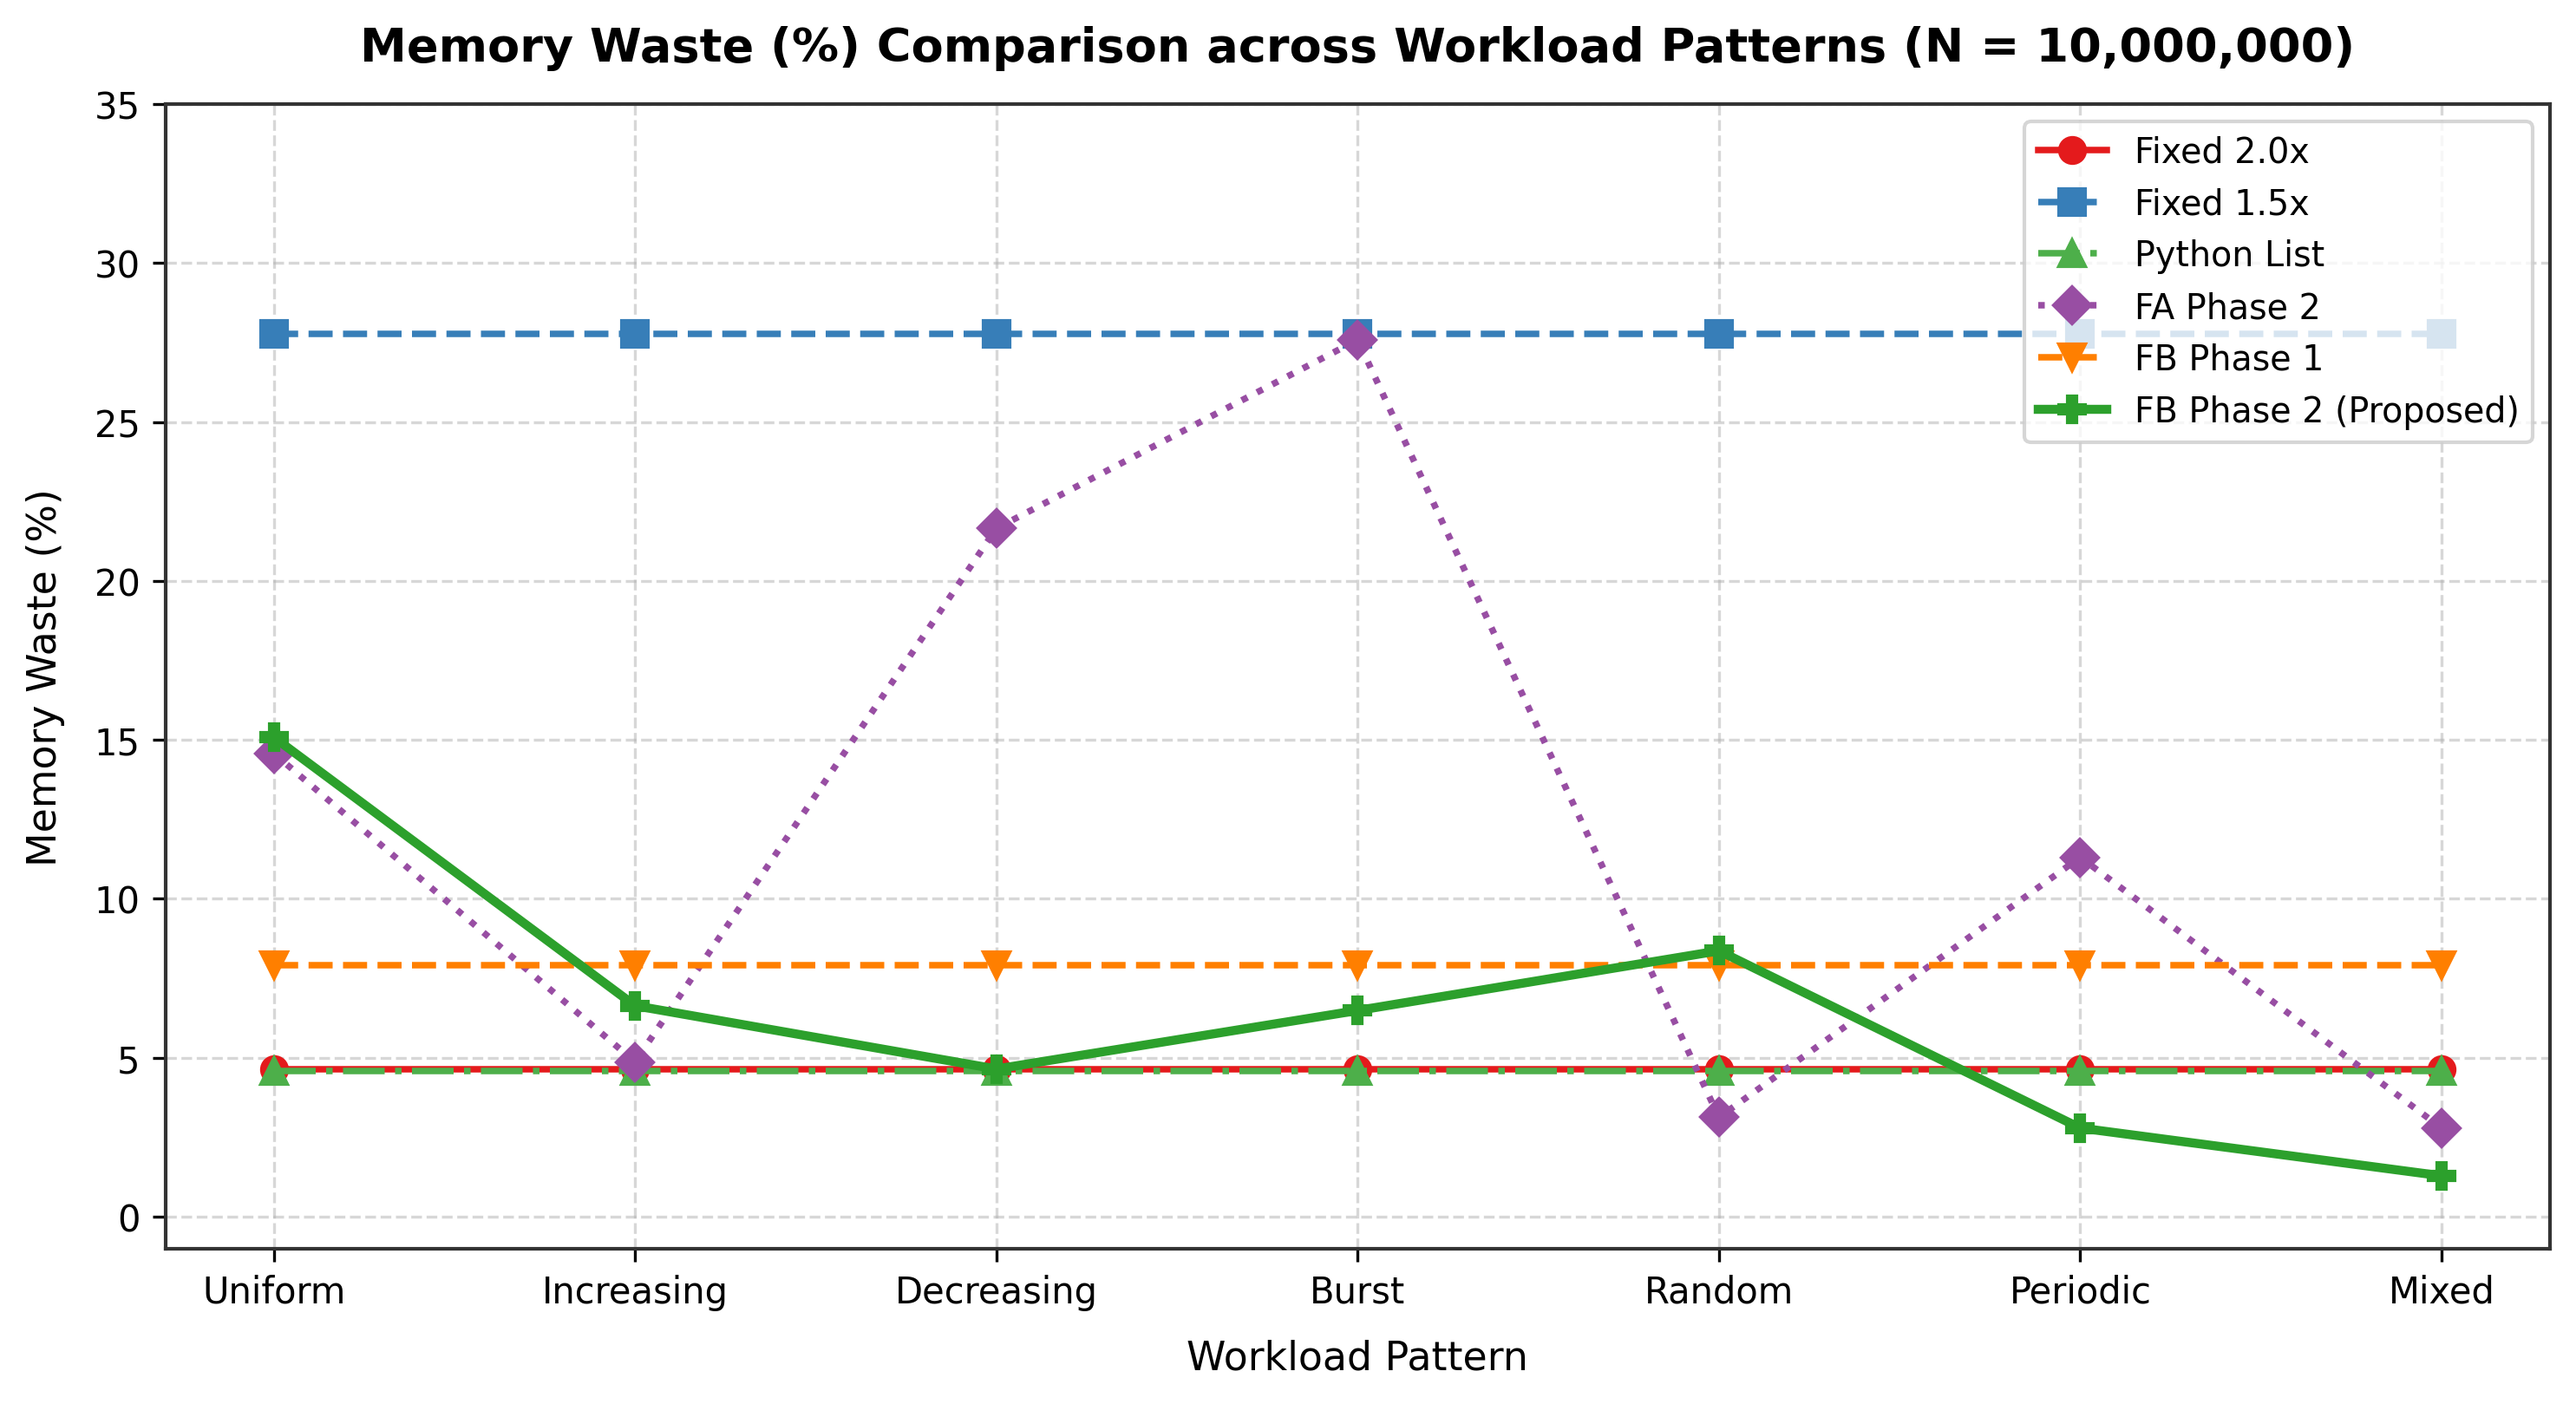
\includegraphics[width=0.75\textwidth]{fb2_combined_patterns_line.png}
\caption{Memory waste percentage comparison across seven workload patterns under $10^7$ insertions.}
\label{fig:memory_waste}
\end{figure}

\section*{Keywords}

Dynamic arrays, Adaptive resizing, Harmonic growth, Workload-aware memory allocation, \mbox{Dynamic} memory management

\section*{References}

\begin{enumerate}[label={[\arabic*]}]

\bibitem{brodnik}
A. Brodnik, S. Carlsson, E. D. Demaine, J. I. Munro, and R. Sedgewick. \textit{Resizable arrays in optimal time and space}. Technical Report CS-99-09, Department of Computer Science, University of Waterloo, 1999.

\bibitem{sartor}
J. B. Sartor, S. M. Blackburn, D. Frampton, M. Hirzel, and K. S. McKinley. Z-rays: divide arrays and conquer speed and flexibility. \textit{Proceedings of the 31st ACM SIGPLAN Conference on Programming Language Design and Implementation (PLDI)}, 471--482, 2010.

\bibitem{bille}
P. Bille, A. R. Christiansen, M. B. Ettienne, and I. L. Gørtz. Fast dynamic arrays. \textit{Proceedings of the 26th Annual European Symposium on Algorithms (ESA)}, 10:1--10:13, 2018.

\end{enumerate}

\end{document}
